% 标准黑白论文版式；报告专用数值与图表不影响展示稿。
\documentclass[11pt,a4paper]{article}
\usepackage[margin=24mm]{geometry}
\usepackage{lmodern,amsmath,amssymb,booktabs,tabularx,array,graphicx,microtype}
\usepackage{xeCJK}
\setCJKmainfont{Noto Serif CJK SC}
\renewcommand{\abstractname}{摘要}
\renewcommand{\figurename}{图}
\renewcommand{\tablename}{表}
\renewcommand{\refname}{参考文献}
\usepackage[font=small,labelfont=bf]{caption}
\usepackage{placeins}
\usepackage[hidelinks]{hyperref}
\pagestyle{plain}
\raggedbottom
\clubpenalty=10000
\widowpenalty=10000
\displaywidowpenalty=10000
\setlength{\parindent}{2em}
\setlength{\parskip}{0pt}
\setlength{\tabcolsep}{5pt}
\renewcommand{\arraystretch}{1.12}
\setcounter{topnumber}{3}
\setcounter{bottomnumber}{2}
\setcounter{totalnumber}{5}
\renewcommand{\topfraction}{.9}
\renewcommand{\bottomfraction}{.8}
\renewcommand{\textfraction}{.08}
\renewcommand{\floatpagefraction}{.8}
\graphicspath{{../results/figures/paper/}}
\newcommand{\PaperMemoryA}{461.6}
\newcommand{\PaperMemoryB}{94.3}
\newcommand{\PaperMemoryC}{94.3}
\newcommand{\PaperMemoryRatio}{4.90}
\newcommand{\PaperTimeB}{0.5442}
\newcommand{\PaperTimeC}{0.5617}
\newcommand{\PaperSERatio}{37.0}
\newcommand{\PaperSEB}{$7.84\times10^{-3}$}
\newcommand{\PaperSEC}{$2.12\times10^{-4}$}
\newcommand{\PaperSmallSEC}{$2.10\times10^{-3}$}
\newcommand{\PaperVarianceRatio}{1,370.6}
\newcommand{\PaperCostRatio}{$7.54\times10^{-4}$}
\newcommand{\PaperCrossTime}{64.36}
\newcommand{\PaperRuntime}{3.49}
\newcommand{\PaperStrikeLowVR}{1,633.9}
\newcommand{\PaperStrikeHighVR}{203.7}
\newcommand{\PaperVolLowVR}{5,231.0}
\newcommand{\PaperVolHighVR}{339.7}
\newcommand{\PaperStepLowTime}{0.0146}
\newcommand{\PaperStepHighTime}{0.3037}
\newcommand{\PaperStepVRMin}{1,347.5}
\newcommand{\PaperStepVRMax}{1,377.0}
\newcommand{\PaperDefaultTable}{\begin{tabular}{llrrrr}
\toprule
路径数 & 方法 & 价格均值 & 标准误 & 种子间标准差 & 耗时（秒） \\
\midrule
$10^{4}$ & A & 5.338061 & $7.83\times10^{-2}$ & $9.41\times10^{-2}$ & 0.0055 \\
 & B & 5.338061 & $7.83\times10^{-2}$ & $9.41\times10^{-2}$ & 0.0055 \\
 & C & 5.362806 & $2.10\times10^{-3}$ & $1.99\times10^{-3}$ & 0.0085 \\
$10^{5}$ & A & 5.366802 & $2.49\times10^{-2}$ & $2.43\times10^{-2}$ & 0.0593 \\
 & B & 5.366802 & $2.49\times10^{-2}$ & $2.43\times10^{-2}$ & 0.0547 \\
 & C & 5.363921 & $6.70\times10^{-4}$ & $7.09\times10^{-4}$ & 0.0591 \\
$10^{6}$ & A & 5.361841 & $7.84\times10^{-3}$ & $6.89\times10^{-3}$ & 0.6105 \\
 & B & 5.361841 & $7.84\times10^{-3}$ & $6.89\times10^{-3}$ & 0.5442 \\
 & C & 5.363854 & $2.12\times10^{-4}$ & $2.73\times10^{-4}$ & 0.5617 \\
\bottomrule
\end{tabular}}
\newcommand{\PaperPilotTable}{\begin{tabular}{rrrrr}
\toprule
预备路径数 & 系数 $\widehat\beta$ & 方差比 & 耗时（秒） & $\eta_C/\eta_B$ \\
\midrule
1,000 & 1.0344 & 1,372.6 & 0.0568 & $7.55\times10^{-4}$ \\
5,000 & 1.0333 & 1,374.1 & 0.0591 & $7.85\times10^{-4}$ \\
10,000 & 1.0333 & 1,374.9 & 0.0620 & $8.24\times10^{-4}$ \\
\bottomrule
\end{tabular}}

\newcommand{\ParallelSerialMs}{543.85}
\newcommand{\ParallelSixMs}{113.39}
\newcommand{\ParallelSpeedup}{4.80}
\newcommand{\ParallelPrice}{5.359797}
\newcommand{\ParallelSE}{0.007842}

\title{\Large\bfseries 基于控制变量的亚式期权高效蒙特卡洛定价}
\author{\normalsize 学号：2026001426}
\date{}
\begin{document}
\maketitle
% 数值来自正式实验记录，表格和图由同一组数据生成。
\begin{abstract}
算术平均亚式期权的到期收益取决于多个观察日的标的价格。
用蒙特卡洛方法定价时，路径存储限制了可模拟的样本规模，抽样误差则限制了估价精度。
本文比较全量向量化、分块模拟和分块加几何控制变量三种方法，并在相同路径上比较串行与多进程执行。
在一百万条正式路径下，分块将峰值常驻内存从 \PaperMemoryA{} MiB 降至 \PaperMemoryB{} MiB。
加入几何控制变量后，标准误中位数降至普通分块的约 \(1/\PaperSERatio\)，单次核心耗时由 \PaperTimeB{} 秒增至 \PaperTimeC{} 秒，后者包含拟合系数的预备计算。
在单独的固定路径对照中，六进程相对于单核串行的实测加速比为 \(\ParallelSpeedup\times\)，两种执行方式得到相同的价格估计与标准误。
改变执行价、波动率和观察次数时，几何控制变量在各组实验中均降低了标准误。
\end{abstract}

\section{引言}
分批采购使企业暴露在一段时间的平均价格风险下。算术平均亚式看涨期权仅在预先约定的观察均价超过执行价时支付差额，因此可为按均价结算的采购提供涨价保护。
估计这份保护今天的价值，需要在价格模型下计算到期收益的折现期望。
蒙特卡洛方法通过生成许多可能的价格路径，计算每条路径的折现收益，再取平均来估计该期望。

模拟规模增大时，保存全部路径的内存随路径数和观察次数一同增长。
同时，标准误通常按独立路径数的平方根倒数下降，若希望将标准误降至原来的十分之一，通常需要约百倍的路径。
分块处理路径可以降低内存占用。利用解析价格已知的几何平均期权作为控制变量，可以减少目标收益中的抽样波动。几何控制变量用于均价期权定价的方法见 Kemna 和 Vorst~\cite{kemna}。

本文在同一路径生成程序下比较全量向量化（A）、分块普通蒙特卡洛（B）和分块加几何控制变量（C）。
A 与 B 的对照衡量存储方式的影响，B 与 C 的对照衡量估计量的影响。
另设一个固定样本对照，将同一批分块路径分别串行与并行计算，评估多进程对耗时的影响。

\section{模型}
\subsection{合约与价格过程}
设 \(S_0\) 为时点零的标的价格，\(K\) 为执行价，\(T\) 为到期时间（年），\(r\) 为常数无风险利率，\(\sigma\) 为常数年化波动率。
合约等间隔观察标的价格 \(m\) 次，观察时点为 \(t_j=jT/m\)，\(j=1,\ldots,m\)。
在风险中性测度 \(\mathbb Q\) 下，假设无分红标的服从几何布朗运动（GBM），其中 \(W_t^{\mathbb Q}\) 为标准布朗运动。
\begin{equation}
dS_t=rS_t\,dt+\sigma S_t\,dW_t^{\mathbb Q}.
\label{eq:gbm}
\end{equation}
记 \((x)_+=\max(x,0)\)，则算术平均看涨期权的折现收益及其理论价格为
\begin{equation}
Y=e^{-rT}\left(\frac1m\sum_{j=1}^{m}S_{t_j}-K\right)_+,
\qquad V_A=\mathbb E^{\mathbb Q}[Y].
\label{eq:target}
\end{equation}
令 \(\Delta t=T/m\)，\(Z_j\) 为相互独立的标准正态变量。在各观察时点采用 GBM 的精确转移：
\begin{equation}
\log S_{t_j}=\log S_{t_{j-1}}+
(r-\sigma^2/2)\Delta t+\sigma\sqrt{\Delta t}\,Z_j.
\label{eq:transition}
\end{equation}

\subsection{几何平均期权}
辅助合约沿用观察时点和执行价。记对数几何均价为 \(L\)，相应折现收益为 \(G\)：
\[
L=m^{-1}\sum_{j=1}^{m}\log S_{t_j},\qquad G=e^{-rT}(e^L-K)_+.
\]
各观察时点的对数价格联合正态，因此 \(L\sim N(\mu_L,v_L)\)，其中
\begin{equation}
\mu_L=\log S_0+(r-\sigma^2/2)\frac{T(m+1)}{2m},
\qquad
v_L=\frac{\sigma^2T(m+1)(2m+1)}{6m^2}.
\end{equation}
这里 \(v_L\) 由布朗运动的协方差 \(\min(t_i,t_j)\) 得到。
令 \(\Phi\) 为标准正态分布函数，记 \(d_2=(\mu_L-\log K)/\sqrt{v_L}\)，\(d_1=d_2+\sqrt{v_L}\)，则几何期权价格为
\begin{equation}
\theta_G=\mathbb E^{\mathbb Q}[G]
=e^{-rT}\left[e^{\mu_L+v_L/2}\Phi(d_1)-K\Phi(d_2)\right].
\label{eq:geometric}
\end{equation}
这一解析期望为后面的控制变量提供了已知基准。

\section{算法}
\subsection{向量化、分块与并行}
记 \(N\) 为正式路径数。方法 A 在 NumPy 数组中一次生成 \(N\times m\) 个正态随机数，累加增量得到对数价格，再计算算术平均期权的折现收益。
方法 B 每次只处理至多 \(b\) 条路径，合并本块的样本数、均值和离均差平方和后释放路径数组~\cite{chan}。
两种方法的计算量均为 \(O(Nm)\)，路径存储由 \(O(Nm)\) 降为 \(O(bm)\)。
A 和 B 使用相同的样本均值估计量。表~\ref{tab:methods} 汇总 A、B、C 的存储和估计方式。

\begin{table}[!htbp]
\centering\small
\caption{三种主实验方法及其比较目的}
\label{tab:methods}
\begin{tabularx}{\linewidth}{lXXX}
\toprule
方法 & 路径存储 & 估计方法 & 比较目的\\
\midrule
A & 完整 \(N\times m\) 数组 & 普通蒙特卡洛 & 全量向量化基准\\
B & 每块至多 \(b\) 条路径 & 普通蒙特卡洛 & 降低路径存储\\
C & 与 B 相同 & 几何控制变量 & 降低抽样方差\\
\bottomrule
\end{tabularx}
\end{table}

在独立的并行对照中，每块的随机流由块编号确定，串行与并行使用相同随机数和路径计算程序。
各工作进程返回本块的样本数、收益均值和离均差平方和。主进程按块编号汇总，再由合并后的统计量计算价格和标准误。

\subsection{控制变量与系数拟合}
方法 C 在同一条模拟路径上计算 \(Y\) 和 \(G\)。
程序先从对数价格求几何均价，再原地转成价格，计算算术平均期权的收益。
对给定系数 \(\beta\)，修正后的收益为
\begin{equation}
X(\beta)=Y-\beta(G-\theta_G).
\end{equation}
因 \(\mathbb E[G-\theta_G]=0\)，有 \(\mathbb E[X(\beta)]=V_A\)。
在 \(\operatorname{Var}(G)>0\) 时，令修正后的收益方差最小可得
\begin{equation}
\beta^*=\frac{\operatorname{Cov}(Y,G)}{\operatorname{Var}(G)}.
\end{equation}
若 \(\rho_{YG}\) 为两种收益的相关系数，则最小方差为
\begin{equation}
\operatorname{Var}\{X(\beta^*)\}=\operatorname{Var}(Y)(1-\rho_{YG}^2).
\label{eq:optimal}
\end{equation}
因此，几何收益与算术收益相关性越强，理论上可消除的抽样波动越多。

总体协方差和方差未知，本文用 \(P\) 条独立预备路径估计系数
\(\widehat\beta=\widehat{\operatorname{Cov}}_{\rm pil}(Y,G)/
\widehat{\operatorname{Var}}_{\rm pil}(G)\)。
在正式样本上固定该系数，估计量为
\begin{equation}
\widehat V_C=\frac1N\sum_{i=1}^N
\left[Y_i-\widehat\beta(G_i-\theta_G)\right].
\label{eq:cv}
\end{equation}
预备样本独立于正式样本，因此 \(\mathbb E[\widehat V_C\mid\widehat\beta]=V_A\)，估计保持无偏。
默认使用 5000 条预备路径。预备样本规模同时影响系数估计的精度和额外计算成本，因此在实验中单独比较。

\subsection{精度与计算成本}
用 \(X_i\) 表示用于估计的收益，即 A、B 的 \(Y_i\) 或 C 的修正收益。记样本均值为 \(\overline X\)，标准误估计为
\begin{equation}
\widehat{\mathrm{SE}}=
\sqrt{\frac{1}{N(N-1)}\sum_{i=1}^N(X_i-\overline X)^2}.
\end{equation}
由正态近似得到 \(\overline X\pm1.96\widehat{\mathrm{SE}}\) 的蒙特卡洛置信区间。

用单次估价耗时 \(t\) 与标准误的平方定义计算成本指标 \(\eta=t\,\widehat{\mathrm{SE}}^2\)。
\(\eta\) 越小，单位时间的估计精度越高。路径数相同时，以 B 和 C 的样本方差之比衡量方差缩减幅度。

\section{数值实验}
\subsection{实验设置}
基准参数为 \(S_0=K=100\)、\(r=0.03\)、\(\sigma=0.20\)、\(T=1\)、\(m=52\)。
主实验使用 \(N\in\{10^4,10^5,10^6\}\)，取 2026 至 2035 共十个独立种子，块大小 \(b=20000\)，预备路径数 \(P=5000\)。
同一设置下，A、B、C 共享正式路径的随机流，C 的预备样本使用独立随机流。
同一种子以相同随机数重复计时三次。价格均值和种子间标准差按每个种子的一次估计计算，耗时与内存使用重复测量；比值先按种子和重复编号配对计算，再取中位数。

单因素敏感性实验使用 \(10^5\) 条正式路径和 2026 至 2030 共五个种子。
依次考察执行价 \(80,100,120\)，波动率 \(0.10,0.20,0.40\)，观察次数 \(12,52,252\)，以及 \(1000,5000,10000\) 条预备路径。其余参数取基准值。

实验在 Intel Core Ultra 9 285K、约 188 GiB 内存的服务器上运行，使用 Python 3.10.19、NumPy 1.26.4 和 SciPy 1.15.3。
主实验和敏感性实验的进程固定在同一个 CPU 核，数值库使用单线程。
每个新进程先用 2048 条路径预热，再重复同种子计算至累计至少 0.2 秒，报告单次估价耗时。
计时包括抽取随机数、模拟路径、计算收益和统计量，以及 C 的预备模拟与几何解析均值计算。导入、预热、文件读写和绘图在计时之外。
峰值常驻内存（RSS）为整个进程的内存峰值，包含解释器、依赖库和预热。
主实验、敏感性实验及绘图共耗时约 \PaperRuntime{} 分钟。

\subsection{基准精度与耗时}
表~\ref{tab:baseline} 汇总价格估计、标准误、种子间波动和耗时。
A 与 B 共用模拟路径，表中的价格估计与标准误相同。
C 的价格估计约为 5.36，单次估计标准误和种子间标准差均明显更小。

\begin{table}[!htbp]
\centering\small
\caption{基准结果。价格均值与种子间标准差基于十个独立估计；标准误和单次耗时均报告中位数。}
\label{tab:baseline}
\PaperDefaultTable
\end{table}

\begin{figure}[!htbp]
\centering
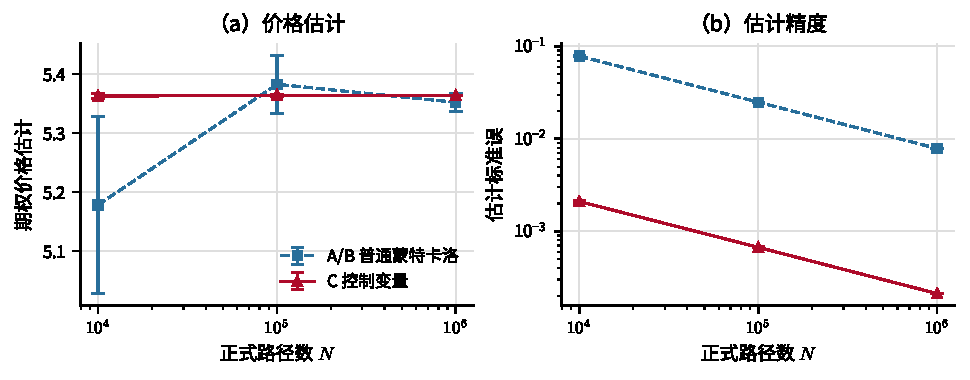
\includegraphics[width=\linewidth]{price_and_se.pdf}
\caption{左：种子 2026 的估计价格及 95\% 蒙特卡洛置信区间。右：十个种子的估计标准误中位数及范围。A 与 B 的曲线重合。}
\label{fig:precision}
\end{figure}

图~\ref{fig:precision} 中，标准误大致随 \(N^{-1/2}\) 下降。
当 \(N=10^6\) 时，B 的标准误中位数为 \PaperSEB{}，C 为 \PaperSEC{}，约降至原来的 \(1/\PaperSERatio\)，配对样本方差比为 \PaperVarianceRatio{}。
同样的路径数下，C 因额外计算几何收益和拟合系数，核心耗时由 B 的 \PaperTimeB{} 秒增至 \PaperTimeC{} 秒。
当 \(N=10^4\) 时，预备路径数占正式路径数的一半，拟合的耗时占比更高。

\subsection{内存与单位时间精度}
图~\ref{fig:memory} 表明，当 \(N=10^6\) 时，A 的峰值 RSS 为 \PaperMemoryA{} MiB，B 和 C 分别为 \PaperMemoryB{} 和 \PaperMemoryC{} MiB，A/B 的比值为 \PaperMemoryRatio{}。
达到块容量后，增加 \(N\) 只增加块数，单块数组不再增大。
计算几何收益时也沿用同样的存储方式。样本较少时，解释器和依赖库在总内存中的占比更大。

\begin{figure}[!htbp]
\centering
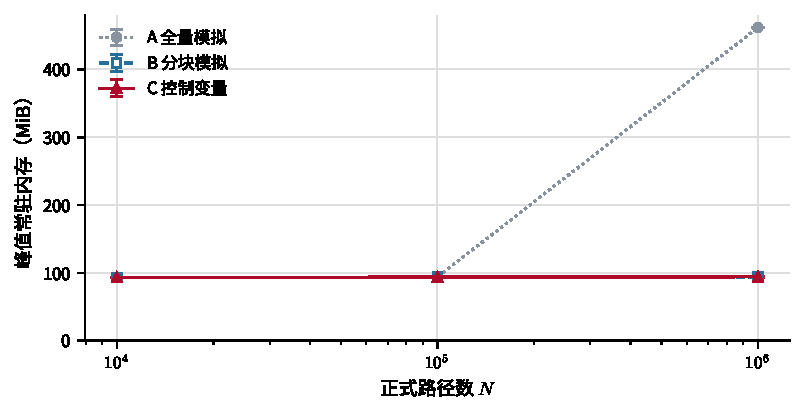
\includegraphics[width=.82\linewidth]{memory_scaling.pdf}
\caption{独立进程峰值 RSS 的中位数和范围。B、C 每块至多 20,000 条路径。}
\label{fig:memory}
\end{figure}

图~\ref{fig:cost} 将耗时和标准误放在同一坐标系下比较。
当 \(N=10^6\) 时，成本指标 \(\eta\) 的 C/B 配对比值为 \PaperCostRatio{}。

进一步比较两种实际配置：C 使用 10,000 条正式路径加 5000 条预备路径，标准误中位数为 \PaperSmallSEC{}；B 使用一百万条路径，标准误中位数为 \PaperSEB{}。
在这两组配置下，配对 B/C 耗时比的中位数为 \PaperCrossTime{}，十个配对种子中 C 的标准误均更小。

\begin{figure}[!htbp]
\centering
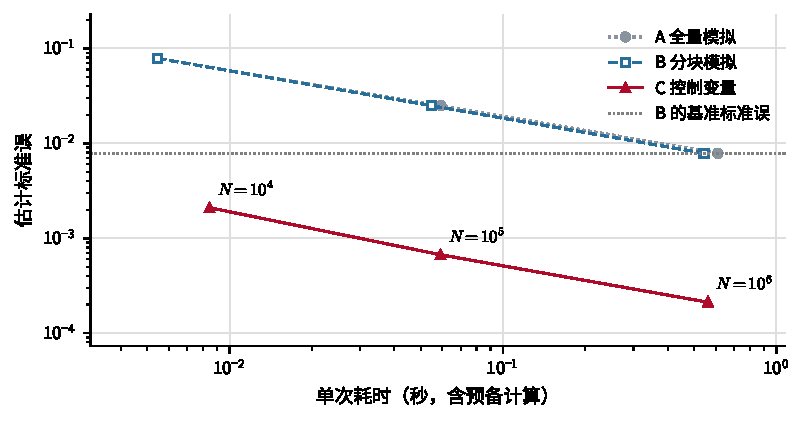
\includegraphics[width=.82\linewidth]{precision_vs_cost.pdf}
\caption{标准误中位数与单次耗时中位数，耗时包含预备计算。虚线为 B 使用 \(10^6\) 条正式路径时的标准误，标记旁为正式路径数。}
\label{fig:cost}
\end{figure}

\subsection{分块并行对照}
分块并行对照沿用方法 B。用种子 2026 生成一百万条路径，分为 50 块，每块 20,000 条。两种执行方式共用各块的随机流。串行固定在一个 CPU 核，并行的六个工作进程共用六核，数值库均为单线程。
两种方式分别预热后计时三次。计时包括任务分发（并行时）、抽取随机数、路径和收益计算以及汇总；进程池初始化和预热在计时之外。

\begin{table}[!htbp]
\centering\small
\caption{同一批路径的串行与并行对照，耗时为三次测量的中位数}
\label{tab:parallel}
\begin{tabular}{lrr}
\toprule
执行方式 & 耗时（毫秒） & 加速比\\
\midrule
单核串行 & \ParallelSerialMs & \(1.00\times\)\\
六进程并行 & \ParallelSixMs & \(\ParallelSpeedup\times\)\\
\bottomrule
\end{tabular}
\end{table}

表~\ref{tab:parallel} 显示，六进程实测加速比为 \(\ParallelSpeedup\times\)。
两种方式得到相同的价格估计 \ParallelPrice{} 和标准误 \ParallelSE{}。

\subsection{合约参数与预备样本敏感性}
图~\ref{fig:sensitivity} 中，C 在各组参数下的标准误均低于 B，方差缩减幅度随合约参数变化。
当 \(K=80\) 和 \(K=120\) 时，配对方差比分别为 \PaperStrikeLowVR{} 和 \PaperStrikeHighVR{}；当 \(\sigma=0.10\) 和 \(\sigma=0.40\) 时，分别为 \PaperVolLowVR{} 和 \PaperVolHighVR{}。
两种均价分处执行价两侧时，几何合约的收益为零，算术合约仍有收益。这类路径会削弱两种收益之间的线性关系。

观察次数从 12 增至 252 时，C 的耗时中位数由 \PaperStepLowTime{} 秒增至 \PaperStepHighTime{} 秒，反映了更多的路径运算。方差比仍处于 \PaperStepVRMin{} 至 \PaperStepVRMax{} 的较窄区间。

\begin{figure}[!htbp]
\centering
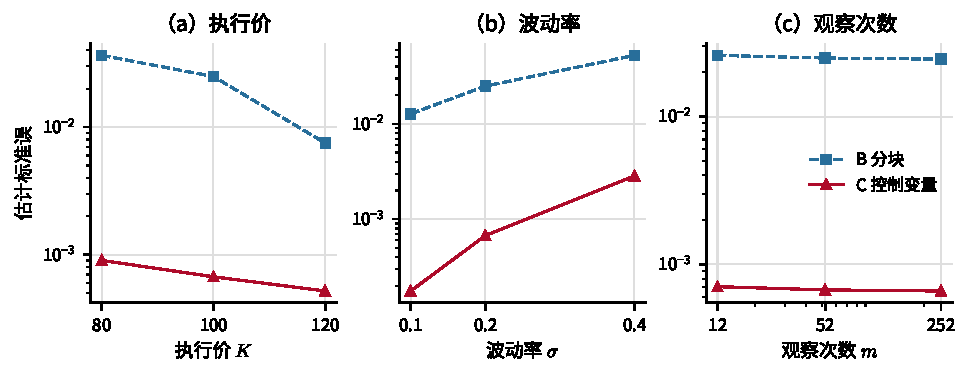
\includegraphics[width=\linewidth]{model_sensitivity.pdf}
\caption{\(N=10^5\) 时五个种子的标准误中位数。每次改变一个参数，其他设定保持基准值。}
\label{fig:sensitivity}
\end{figure}

\begin{table}[!htbp]
\centering\small
\caption{\(N=10^5\) 和五个种子下的预备样本敏感性。系数和耗时报告中位数，方差比和精度成本比与 B 配对计算。}
\label{tab:pilot}
\PaperPilotTable
\end{table}

\FloatBarrier
\section{结论}
分块模拟用块大小控制路径存储，并保留普通蒙特卡洛的样本均值。几何控制变量降低了单条路径的收益方差，使较少的正式路径也能取得较小的标准误。固定路径的实验中，六进程并行将分块模拟的耗时缩短至单核串行的约 \(1/\ParallelSpeedup\)。

在本文的几何布朗运动模型下，几何平均期权的解析价给出了控制变量的期望。将同一估计式用于其他价格模型时，需要获得相应辅助收益的期望。

\begin{thebibliography}{9}\small\raggedright
\bibitem{kemna}
A. G. Z. Kemna and A. C. F. Vorst.
A pricing method for options based on average asset values.
\textit{Journal of Banking \& Finance}, 14(1):113--129, 1990.
\href{https://doi.org/10.1016/0378-4266(90)90039-5}{doi:10.1016/0378-4266(90)90039-5}.
\bibitem{chan}
T. F. Chan, G. H. Golub, and R. J. LeVeque.
Algorithms for computing the sample variance: Analysis and recommendations.
\textit{The American Statistician}, 37(3):242--247, 1983.
\href{https://doi.org/10.1080/00031305.1983.10483115}{doi:10.1080/00031305.1983.10483115}.
\end{thebibliography}

\end{document}
